\chapter{Design}

I dette kapitel vil vi gennemgå spillet design, og vi vil vise et flow-, klasse- og system sekvensdiagram.

\pagebreak
\section{Flowdiagram}
Indledningsvis tegnede vi et flowdiagram for at skabe overblik over projektet, så vi kunne forstå, hvordan spillet skulle udføres.
Flowdiagrammet blev brugt som baggrund for de efterfølgende diagrammer, som bliver vist i projektet.

\begin{center}
\begin{tikzpicture}[node distance=2cm]
    \node (start) [startstop] {Spillet startes};
    \node (kast) [process, below of=start] {Terningerne kastes};
    \node (passeres) [decision, below of=kast] {Passeres start?};
    \node (ejendom) [decision, below of=passeres, yshift=-1cm] {Er feltet en ejendom?};
    \node (chance) [decision, below of=ejendom, yshift=-1cm] {Er feltet chance?};
    \node (stash) [decision, left of = chance, xshift =-1cm] {Stash \begin{math}
        \geq
    \end{math} ejendomsværdi};
    \node (ejer) [decision, left of = ejendom, xshift = -1cm] {Ejes ejendommen?};
    \node (koeb) [process, left of = ejer, xshift = -2.5cm] {Koeb ejendom};
    \node (betal) [process, left of = passeres, xshift = -2cm] {Betal leje};
    \node (penge) [process, right of = passeres, yshift =-1.9cm, xshift = 0.7cm] {Få penge};
    \node (instrukser) [process, right of = chance, xshift=2.5cm] {Følg instrukser};
    \node (slut) [startstop, left of = stash, xshift =-2.5cm] {Spillet sluttes}; 
    \draw [arrow] (start) -- (kast);
    \draw [arrow] (kast) -- (passeres);
    \draw [arrow] (passeres) -| node[anchor=south] {Ja} (penge);
    \draw [arrow] (passeres) -- node[anchor=west] {Nej}  (ejendom);
    \draw [arrow] (penge) |- (ejendom);
    \draw [arrow] (ejendom) -- node[anchor=south] {Ja} (stash);
    \draw [arrow] (ejendom) -- node[anchor=west] {Nej} (chance);
    \draw [arrow] (chance) -- node[anchor=south] {Ja} (instrukser);
    \draw [arrow] (stash) --node[anchor=west] {Ja} (ejer);
    \draw [arrow] (stash) --node[anchor=south] {Nej} (slut);
    \draw [arrow] (ejer) --node[anchor=south] {Nej} (koeb);
    \draw [arrow] (koeb) |- (kast);
    \draw [arrow] (ejer) -- node[anchor=west] {Ja} (betal);
    \draw [arrow] (betal) |- (kast);
    \draw [arrow] (instrukser) |- (kast);
    \end{tikzpicture}
\end{center}



\section{Klassediagram}

\section{Systemsekvens diagram}
\begin{figure}[H]
    \begin{center}
        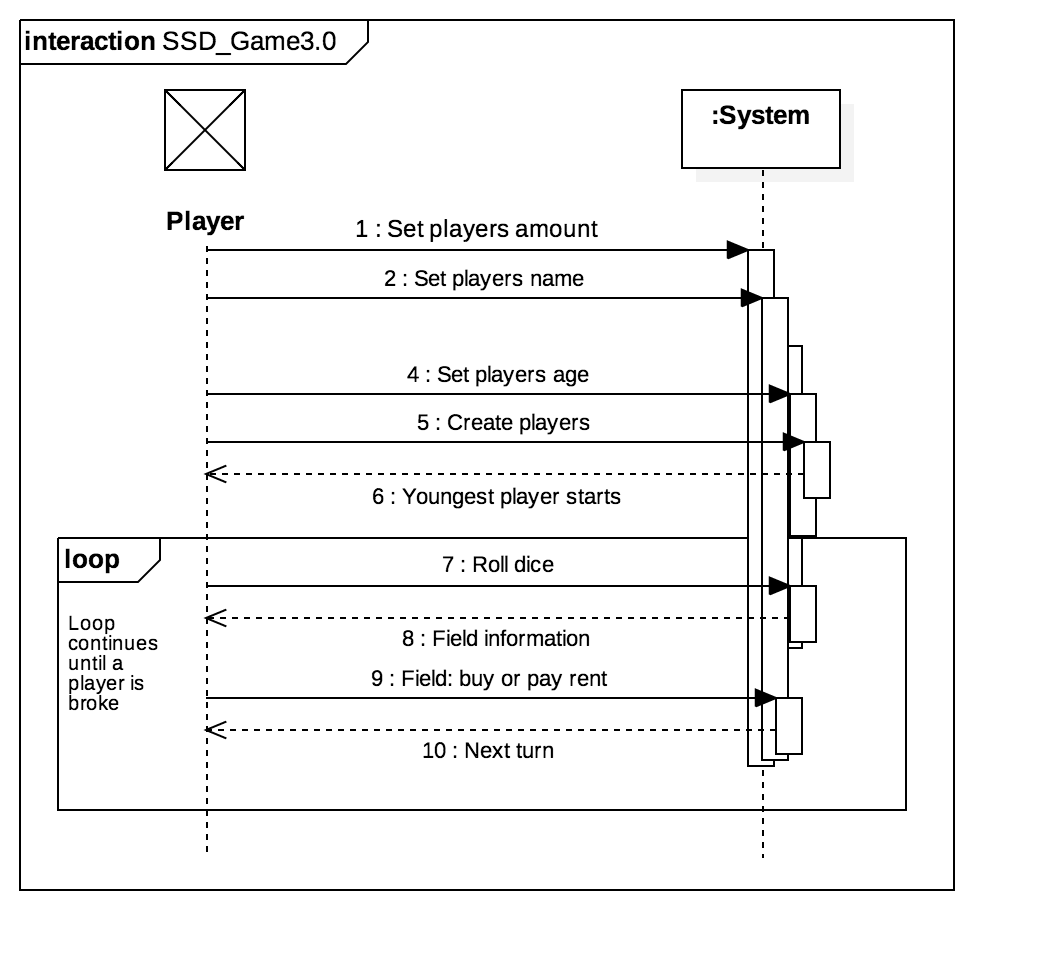
\includegraphics[width=\columnwidth]{graphics/domain/SSD_Game3.png}
        \caption{Systemsekvens diagram}
        \label{fig:systemsekvens_diagram}
    \end{center}
\end{figure}

\section{Sekvens diagram}
\begin{figure}[H]
    \begin{center}
        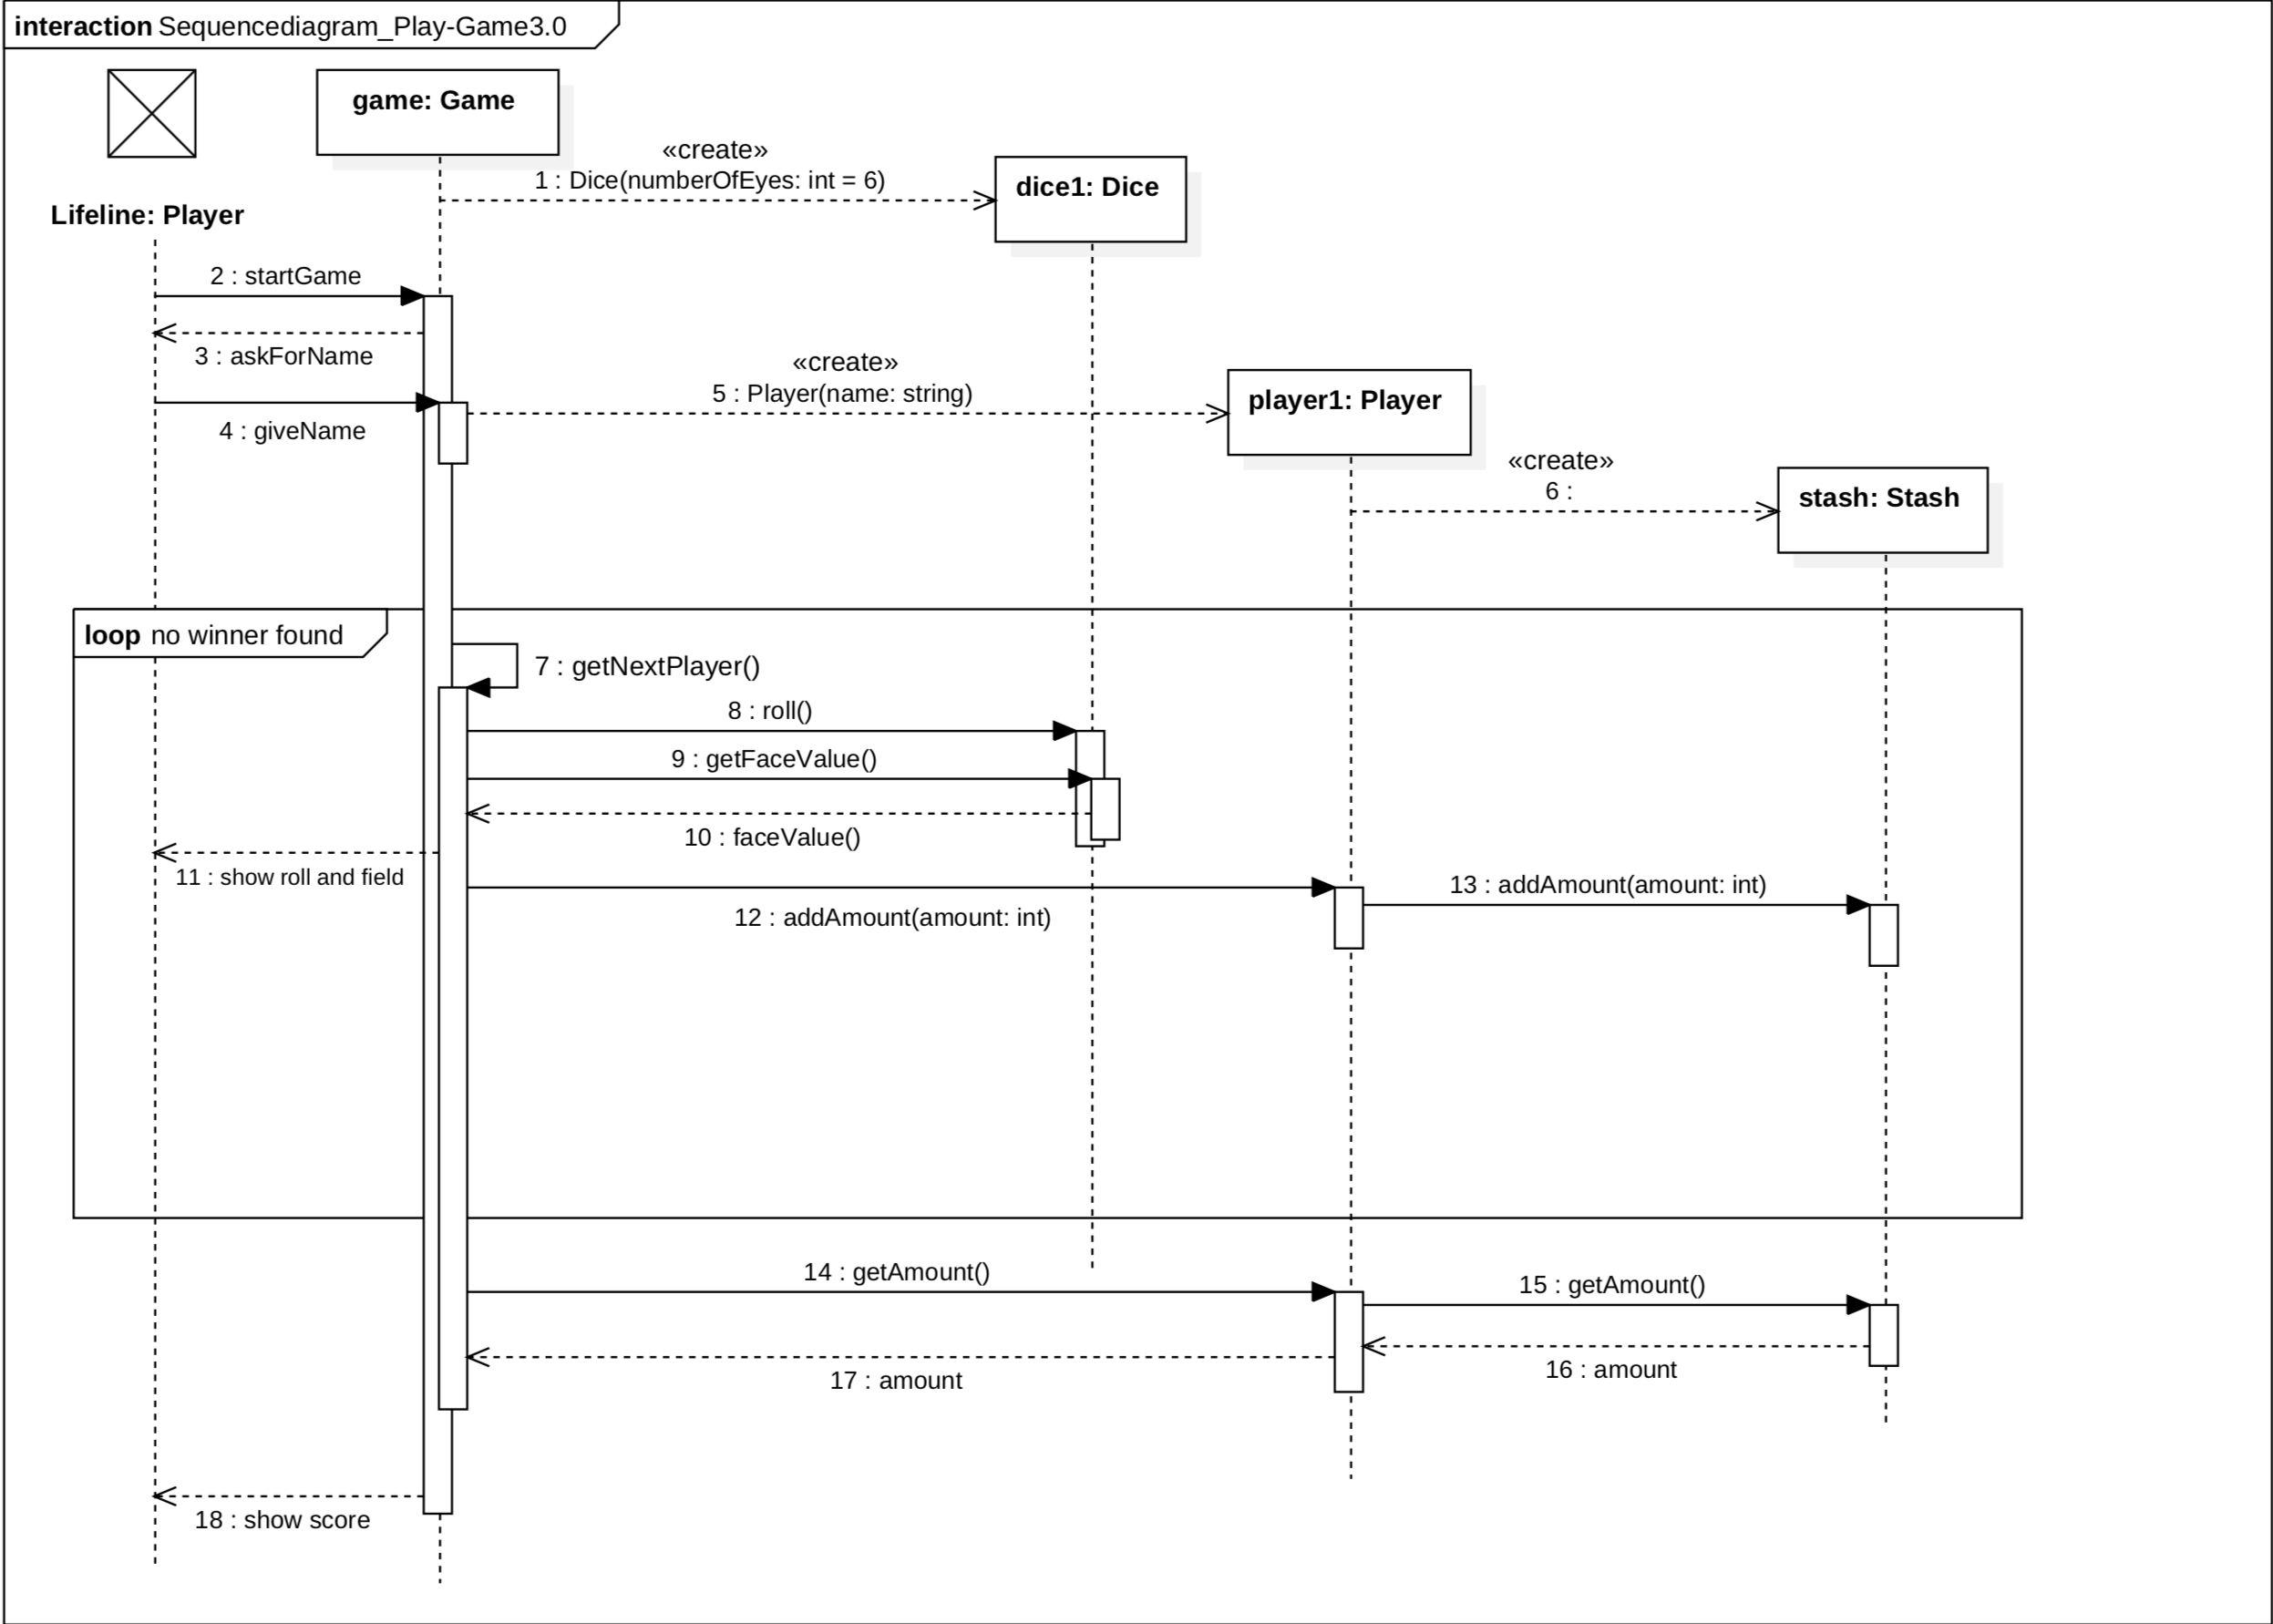
\includegraphics[width=\columnwidth]{graphics/domain/SD_Game3.png}
        \caption{Sekvens diagram}
        \label{fig:sekvens_diagram}
    \end{center}
\end{figure}